\documentclass[12pt,landscape,letterpaper]{article}
\usepackage{multicol}
\usepackage{calc}
\usepackage[top=.25in,left=.25in,right=.25in,bottom=.25in]{geometry}
\usepackage{amsmath,amsthm,amsfonts,amssymb}
\usepackage{hyperref}
\usepackage{enumitem}
\usepackage{upgreek}
\usepackage{physics}
\usepackage{mathtools}
\usepackage{newtxtext,newtxmath}
\usepackage{booktabs}
\usepackage{xfrac}
\usepackage{graphicx}
\usepackage{tabularx}

% Images in the images directory
\graphicspath{ {./images/} }

% Turn off header and footer
\pagestyle{empty}
 

% Redefine section commands to use less space
\makeatletter
\renewcommand{\section}{\@startsection{section}{1}{0mm}%
                                {-1ex plus -.5ex minus -.2ex}%
                                {0.5ex plus .2ex}%x
                                {\normalfont\normalsize\bfseries}}
\renewcommand{\subsection}{\@startsection{subsection}{2}{0mm}%
                                {-1explus -.5ex minus -.2ex}%
                                {0.5ex plus .2ex}%
                                {\normalfont\small\bfseries}}
\renewcommand{\subsubsection}{\@startsection{subsubsection}{3}{0mm}%
                                {-1ex plus -.5ex minus -.2ex}%
                                {1ex plus .2ex}%
                                {\normalfont\footnotessize\bfseries}}
\makeatother

% Don't print section numbers
\setcounter{secnumdepth}{0}

\setlength{\parindent}{0pt}
\setlength{\parskip}{1pt plus 0.5ex}

\newcommand{\tab}{\hspace{0.02\textwidth}}
\newcommand{\tabm}{\hspace*{0.07\textwidth}}
\newcommand{\ds}{\displaystyle}

\renewcommand{\dv}[2]{\frac{d#1}{d#2}}
\DeclareMathOperator{\sinc}{sinc}
\DeclareMathOperator{\rect}{rect}

% -----------------------------------------------------------------------

\begin{document}

\raggedright
\footnotesize
\begin{multicols*}{3}


% multicol parameters
% These lengths are set only within the two main columns
%\setlength{\columnseprule}{0.25pt}
\setlength{\premulticols}{1pt}
\setlength{\postmulticols}{1pt}
\setlength{\multicolsep}{1pt}
\setlength{\columnsep}{2pt}

\begin{center}
	\Large{\underline{ELEC 221 Formula Sheet}}\\
	\small{From Ryan M. and Donney F.}
\end{center}

\section{Continuous Time Signals}

Even and Odd Components:\\
\tab $\ds x_e(t) = \frac{1}{2}[x(t) + x(-t)]$\\
\tab $\ds x_o(t) = \frac{1}{2}[x(t) - x(-t)]$

A signal is periodic with fundamental period $T_0$ if\\
\tab $x(t + kT_0) = x(t) \quad \forall t \in (-\infty, \infty)$

Energy:\\
\tab $\ds E = \int_{-\infty}^{\infty} \abs{x(t)}^2\,dt$\\
\tab Energy of a sinusoid is always infinite\\
Power:\\
\tab $\ds P = \lim_{T \rightarrow \infty} \frac{1}{2T} \int_{-T}^{T}\abs{x(t)}^2\,dt$

Causality:\\
\begin{itemize}
	\itemsep0em
	\item Causal: $x(t) = 0$ for $t < 0$.
	\item Anti-Causal: $x(t) = 0$ for $t \geq 0$.
	\item A-Causal or Non-Causal: Both of the above.
\end{itemize}

\section{Continuous Time Systems}
Dynamic systems have memory. Active systems can deliver energy to the outside world.
\\
Linearity:\\
\tab $\mathcal{S}[\alpha x(t) + \beta y(t)] = \alpha\mathcal{S}[x(t)] + \beta\mathcal{S}[y(t)]$

Time Invariance:\\
\tab If $\mathcal{S}[x(t)] = y(t)$ then $\mathcal{S}[x(t \pm \tau)] = y(t \pm \tau)$.

Zero-State Response:\\
\tab Due to the input as the initial conditions are zero.

Zero-Input Response:\\
\tab Due to the initial conditions as the input is zero.

Convolution:\\
\tab $\ds y(t) = \int_{-\infty}^{\infty}x(\tau)h(t-\tau)\,d\tau$

Causality:\\
\tab A continuous time system $\mathcal{S}$ is causal if whenever $x(t) = 0$ and there are no initial conditions, $y(t) = 0$ and the output $y(t)$ does not depend on future inputs.
\\~\\
Bounded-Input Bounded-Output Stability:\\
\tab If an input $x(t)$ bounded then the output of an BIBO system is also bounded.\\
\tab $\ds \int_{-\infty}^{\infty} \abs{h(t)}\,dt < \infty$

\section{Laplace Transform}
$s = \sigma + j\omega$\\

Eigenfunction Property:\\
\tab $\mathcal{S}[e^{s_0t}] = H(s_0)e^{s_0t}$

One Sided Laplace Transform:\\
\tab $\ds F(s) = \mathcal{L}[f(t)u(t)] = \int_{0^-}^{\infty}f(t)e^{-st}\,dt$\\
\tab $\abs{H(s)}$ is greatest when $\omega$ is closest to the poles.

\begin{tabular}{ll}  
	\toprule
	Signal Support & ROC\\
	\midrule
	Finite support & Entire s-plane.\\
	Causal function & $\sigma > \max(\sigma_i)$,  $-\infty < \omega < \infty$\\
	Anti-causal & $\sigma < \min(\sigma_i)$,  $-\infty < \omega < \infty$\\
	Non-causal & $\mathcal{R} = \mathcal{R}_\text{causal} \cap \mathcal{R}_\text{anti-causal}$\\
	\bottomrule
\end{tabular}
\vspace{0.5em}

Initial Value Theorem:\\
\tab $\ds f(0+) \Leftrightarrow \lim_{s\rightarrow\infty} sF(s)$

Final Value Theorem:\\
\tab $\ds \lim_{t\rightarrow\infty} f(t) \Leftrightarrow \lim_{s\rightarrow 0} sF(s)$

Bounded-Input Bounded-Output Stability:\\
\tab If the region of convergence contains the $j\omega$-axis, then the system is BIBO stable.

\section{Fourier Series}
\tab Fourier analysis in the steady state.

Eigenfunction Property:\\
\tab $\mathcal{S}[e^{j\omega_0t}] = H(j\omega_0)e^{j\omega_0t}$\\
\tab $x(t) = \sum_k X_k e^{j\omega_kt} \implies y(t) = \sum_k X_k H(j\omega_k)e^{j\omega_kt}$\\\vspace{1mm}\hspace{2.5cm}$= \sum_k X_k \abs{H(j\omega_k)}e^{j(\omega_kt + \angle H(\omega_k))}$

Fourier Series Coefficients (for any $t_0$):\\
\tab $\ds X_k = \frac{1}{T_0}\int_{t_0}^{t_0 + T_0}x(t)e^{-jk\omega_0t}\,dt$

Parseval's Power Relation (for any $t_0$):\\
\tab $\ds P = \frac{1}{T_0} \int_{t_0}^{t_0 + T_0}\abs{x(t)}^2\,dt = \sum_{k = -\infty}^{\infty}\abs{X_k}^2$

Symmetry of Line Spectra:\\
\tab $\abs{X_k} = \abs{X_{-k}}$\\
\tab $\angle X_k = -\angle X_{-k}$

Trigonometric Fourier Series:\\
\tab $x(t) = X_0 + 2\sum_{k = 1}^{\infty}\abs{X_k}\cos(k\omega t + \Theta_k)$\\
\tab $x(t) = c_0 + 2\sum_{k = 1}^{\infty}[c_k\cos(k\omega_0 t) + d_k\sin(k\omega_0 t)]$\\
\tab $c_k = \frac{1}{T_0} \int_{t_0}^{t_0 + T_0}x(t)\cos(k\omega_0 t)\,dt$ \quad $k$ = 0,1,2$\ldots$\\
\tab $d_k = \frac{1}{T_0} \int_{t_0}^{t_0 + T_0}x(t)\sin(k\omega_0 t)\,dt$\quad $k$ = 1,2,3$\ldots$\\
\tab $\Theta_k = -\arctan(d_k/c_k)$

\columnbreak
Fourier Coefficients from Laplace Transform:\\
\tab If $x_1(t)$ is a single period of $x(t)$, then\\
\tab $X_k = \frac{1}{T_0}\mathcal{L}[x_1(t)] \big\rvert_{s = jk\omega_0}$

Response of LTI Systems to Periodic Signals:\\
\tab If the input to an LTI system has Fourier Series $x(t) = X_0 + 2\sum_{k=1}^{\infty}\abs{X_k}\cos(k\omega t + \angle X_k)$, then the steady state response is $\ds y(t) = X_0\abs{H(j0)} + 2\sum_{k=1}^{\infty}\abs{X_k}\abs{H(jk\omega_0)}\cos(k\omega_0 t + \angle X_k + \angle H(jk\omega_0))$

\section{Fourier Transform}
\tab $X(\omega) = \int_{-\infty}^{\infty}x(t)e^{-j\omega t}\,dt$\\
\tab $x(t) = \frac{1}{2\pi}\int_{-\infty}^{\infty}X(\omega)e^{j\omega t}\,d\omega$

Fourier Transform from Laplace Transform (if $X(s)$ contains the $j\omega$-axis):\\
\tab $\mathcal{F}[x(t)] = \mathcal{L}[x(t)]\big\rvert_{s = j\omega} = X(s)\big\rvert_{s = j\omega}$

Fourier Transform of Periodic Signals:\\
\tab $\ds \sum_k X_k e^{jk\omega_0 t} \xLeftrightarrow{\mathcal{F}} \sum_k 2\pi X_k \delta(\omega - k\omega_0)$

Parseval's Energy Relation:\\
\tab $\ds E = \int_{-\infty}^{\infty} \abs{x(t)}^2\,dt = \frac{1}{2\pi}\int_{-\infty}^{\infty}\abs{X(\omega)}^2\,d\omega$

Symmetry of Spectral Representations:\\
\tab $\abs{X(\omega)} = \abs{X(-\omega)}$\\
\tab $\Re[X(\omega)] = \Re[X(-\omega)]$\\
\tab $\angle X(\omega) = -\angle X(-\omega)$\\
\tab $\Im[X(\omega)] = -\Im[X(-\omega)]$

\section{Sampling Theory}
\tab $x_s(t) = x(nT_s) = x(t)\rvert_{t = nT_s} = x(t)\sum_n \delta(t - nT_s)$\\
\tab $\ds X_s(\omega) = \frac{1}{T_s} \sum_{k=-\infty}^{\infty}X(\omega - k\omega_s)$

Nyquist-Shannon Sampling Rate:\\
\tab $\omega_s = \frac{2\pi}{T_s} \geq 2\omega_\text{max}$\\
\tab Aliasing occurs if $\omega_s < 2\omega_\text{max}$.

Reconstruction $X(\omega)=X_s(\omega)H_\text{lp}(\omega)$:
\vspace{-1em}
\begin{equation*}
\hspace{-8em}
H_{\text{lp}}(\omega) =
\begin{cases}
T_s & \ds -\frac{\omega_s}{2} \leq \omega \leq \frac{\omega_s}{2}\\
0 & \text{otherwise}
\end{cases}
\end{equation*}
\tab (Inclusive bounds. If represented by a unit step function the bounds are inclusive for filters (Refer to lecture notes))

Signal Reconstruction from Sinc Interpolation:\\
\tab $\ds x_r(t) = \sum_{n=-\infty}^{\infty} x(nT_s) \frac{\sin(\pi(t-nT_s)/T_s)}{\pi(t-nT_s)/T_s}$
\end{multicols*}

\newpage

\begin{minipage}[t]{0.27\textwidth}
\section{Discrete Time Signals}
\tabm Define $x[n] = x(nT_0)$.\\
\tabm $x[n] = \sum_{k=-\infty}^{\infty}x[k]\delta[n-k]$

Periodicity:\\
\tabm $x[n + kN] = x[n]$ \qquad $\forall k\in \mathbb{Z}$

When sampling an analog sinusoid of fundamental period $T_0$, we obtain a periodic discrete sinusoid provided that $m$, $N$ not divisible by each-other:\\
\tabm $T_s/T_0 = m/N$

Aliasing occurs if:\\
\tabm $T_s > T_0/2$

Energy:\\
\tabm $\ds E = \sum_{n = -\infty}^{\infty}\abs{x[n]}^2$

Power:\\
\tabm $\ds P_x = \lim_{N \rightarrow \infty}\frac{1}{2N + 1}\sum_{n= -N}^{N}\abs{x[n]}^2$

Convolutional Sum:\\\
\tabm $\ds y[n] = \sum_{k = -\infty}^{\infty} x[k]h[n-k]$

Bounded-Input Bounded-Output Stability:\\
\tabm $\sum_k \abs{h[n]} < \infty$

Solution to Autoregressive Discrete System:\\
\tabm $y[n] = ay[n-1] + bx[n]$, $n \geq 0$\\
\tabm $y[n] = \sum_{k=0}^{n} ba^kx[n-k]$, $n\geq 0$

\section{Z-Transform}
\tabm $\mathcal{Z}[x(nT_s)] = \mathcal{L}[x_s(t)]\rvert_{z=e^{sT_s}} = \sum_n x(nT_s)z^{-n}$

Convergence:\\
\tabm $|X(z)| = \sum_n \abs{x[n]}r^{-n} < \infty$

Initial Value Theorem:\\
\tabm $\ds x[0] = \lim_{z\rightarrow \infty}X(z)$

Final Value Theorem:\\
\tabm $\ds \lim_{n\rightarrow \infty}x[n] = \lim_{z\rightarrow 1}(z-1)X(z)$

BIBO Stability:\\
\tabm If the ROC contains radius $z=1$, then the system is BIBO stable.

\section{Misc. Identities}
\tabm $\ds \sum_{k=0}^{n}x^k = \frac{1-x^{n+1}}{1-x} \quad\xrightarrow{n\rightarrow\infty \text{ and } x < 1}\quad \frac{1}{1-x}$\\
\tabm $\ds \cos\theta = \frac{e^{j\theta}+e^{-j\theta}}{2}$\\
\tabm $\ds \sin\theta = \frac{e^{j\theta}-e^{-j\theta}}{2j}$

% Footer content
\rule{0.3\linewidth}{0.25pt}
\scriptsize\\
Updated \today\\
\href{https://github.com/sgoblin/elec221-formulasheet}{https://github.com/sgoblin/elec221-formulasheet}
\end{minipage}%
\hspace{0.5em}
\begin{minipage}[t]{0.35\textwidth}
\subsection{Partial Fraction Decomposition}
\begin{tabular}{lll}  
	\toprule
	Fraction & Partial Fraction & Solution\\
	\midrule\vspace{1mm}
	$\ds \frac{px + q}{(x-a)(x-b)}$ & $\ds \frac{A}{x-a} + \frac{B}{x-b}$ & $\ds A = \dfrac{pa + q}{a-b} \quad B =\dfrac{pb + q}{b-a}$\\\vspace{1mm}
	$\ds \frac{px + q}{(x-a)^2}$ & $\ds \frac{A}{x-a} + \frac{B}{(x-a)^2}$  & $\ds A = p \qquad\quad B = pa + q$\\\vspace{1mm}
	$\ds \frac{px^2 + qx + r}{(x-a)(x-b)(x-c)}$ & $\ds \frac{A}{x-a} + \frac{B}{x-b} + \frac{C}{x-c}$    & $A=\dfrac{pa^2 + qa +r}{(a-b)(a-c)} \quad B =\dfrac{pb^2 + qb +r}{(b-a)(b-c)} \quad C =\dfrac{pc^2 + qc +r}{(c-a)(c-b)}$\\\vspace{1mm}
	$\ds \frac{px^2 + qx + r}{(x-a)^2(x-b)}$ & $\ds \frac{A}{x-a} + \frac{B}{(x-a)^2} + \frac{C}{x-b}$ & \\\vspace{1mm}
	$\ds \frac{px^2 + qx + r}{(x-a)(x^2 + bx + c)}$ & $\ds \frac{A}{x-a} + \frac{Bx + C}{x^2 + bx + c}$ &\\
	\bottomrule
\end{tabular}
\vspace{0.5em}
\subsection{Two-Sided Z-Transforms}
\begin{tabular}{lll}  
	\toprule
	$f[n]$ & $F(z)$ & ROC\\
	\midrule\vspace{1mm}
	$-u[-n-1]$ & $\ds \frac{1}{1-z^{-1}}$ & $\abs{z} < 1$\\\vspace{1mm}
	$-\alpha^nu[-n-1]$ & $\ds \frac{1}{1-\alpha z^{-1}}$ & $\abs{z} < \abs{\alpha}$\\\vspace{1mm}
	$-n\alpha^nu[-n-1]$ & $\ds \frac{\alpha z^{-1}}{(1-\alpha z^{-1})^2}$ & $\abs{z} < \abs{\alpha}$\\\vspace{1mm}
	$\alpha^\abs{n}$, $\abs{\alpha} < 1$ & $\ds \frac{1}{1-\alpha z^{-1}} - \frac{1}{1-\alpha^{-1} z^{-1}}$ & $\abs{\alpha} < z < \abs{\frac{1}{\alpha}}$\\
	\bottomrule
\end{tabular}
\vspace{0.5em}
\subsection{Interconnection of LTI Systems}
\begin{tabular}{lll}  
	\toprule
	Connection & Time & Laplace/Z\\
	\midrule\vspace{1mm}
	Series & $[h_1 * h_2](t)$ & $H_1(s)H_2(s)$\\
	Parallel & $h_1(t) + h_2(t)$ & $H_1(s) + H_2(s)$\\
	\bottomrule
\end{tabular}

\subsection{Misc. More}

\[\int_{-\infty}^{\infty} e^{-a(x+b)^2} dx = \sqrt{\frac{\pi}{a}}\]


\end{minipage}
\begin{minipage}[t]{0.30\textwidth}
	\vspace{18em}
	\subsection{Finding Magnitudes}
	\tabm If $\ds H(s) = \frac{N(s)}{D(s)}$, then $\ds \abs{H(s)} = \frac{\abs{N(s)}}{\abs{D(s)}} = \frac{\sqrt{(N(s))^2}}{\sqrt{(D(s))^2}}$\\
	and $\angle H(s) = \angle N(s) - \angle D(s)$
	
	Complex Valued:\\
	\tabm $\abs{H(s)}^2 = H(s)H(s)^*$
	
	\subsection{Long Division For Z-Transform Inverse}
	Let $X(z) = B(z)/A(z)$ be a rational Z-Transform of a causal signal $x[n]$. We can then express $X(z)$ as
	$$X(z) = x[0] + x[1]z^{-1} + x[2]z^{-2} + \cdots$$
	by dividing $B(z)$ by $A(z)$. To perform the long division, we let $X(z)$ be the series of $z^{-n}$ as above, and multiply both sides throiugh by $A(z)$ to obtain $A(z)X(z) = B(z)$. We then compare the coefficients in front of $z^{-n}$ of both sides to obtain values for the sequence $\{x[0], x[1], x[2], x[3], \ldots\}$. Then the inverse can be taken by inspection.
	
	\subsection{Fourier Transform of a Periodic Signal}
	Suppose $x(t)$ is periodic of period $T_0$. Let $x_p(t)$ be a single period of $x(t)$. Then $x(t) = \sum_k x_p(t - kT_0)$ and we can find $X(\omega)$ by using time shifting property and finding the Fourier Transform of $x_p(t)$ by using Laplace.
\end{minipage}
\newpage

\begin{multicols*}{3}
	% multicol parameters
	% These lengths are set only within the two main columns
	%\setlength{\columnseprule}{0.25pt}
	\setlength{\premulticols}{1pt}
	\setlength{\postmulticols}{1pt}
	\setlength{\multicolsep}{1pt}
	\setlength{\columnsep}{2pt}
	
	\section{Periodicity}
	Sum or product of periodic functions with periods $T_1$ and $T_2$ is periodic iff $\frac{T_1}{T_2} = \frac{n_1}{n_2}$ where $n_1$ and $n_2$ are integers.\\
	Period of sum/product:\\
	\tab LCM($T_1$,$T_2$)\\
	
	\section{Trigonometric Identities}
	\[1+tan^2\theta=sec^2\theta\]
	\[1+cot^2\theta = csc^2\theta\]
	\[sin(A\pm B) = sin(A)cos(B)\pm cos(A)sin(B)\]
	\[cos(A\pm B) = cos(A)cos(B)\mp sin(A)sin(B)\]
	\[sin(2\theta)=2sin(\theta)cos(\theta)\]
	\[cos(2\theta)=cos^2\theta - sin^2\theta = 2cos^2\theta - 1 = 1-2sin^2\theta\]
	\[tan(2\theta)=\frac{2tan(\theta)}{1-tan^2(\theta)}\]
	\[cos(\theta)=sin(\theta +\frac{\pi}{2})\]
	
	\section{Unit Circle}
	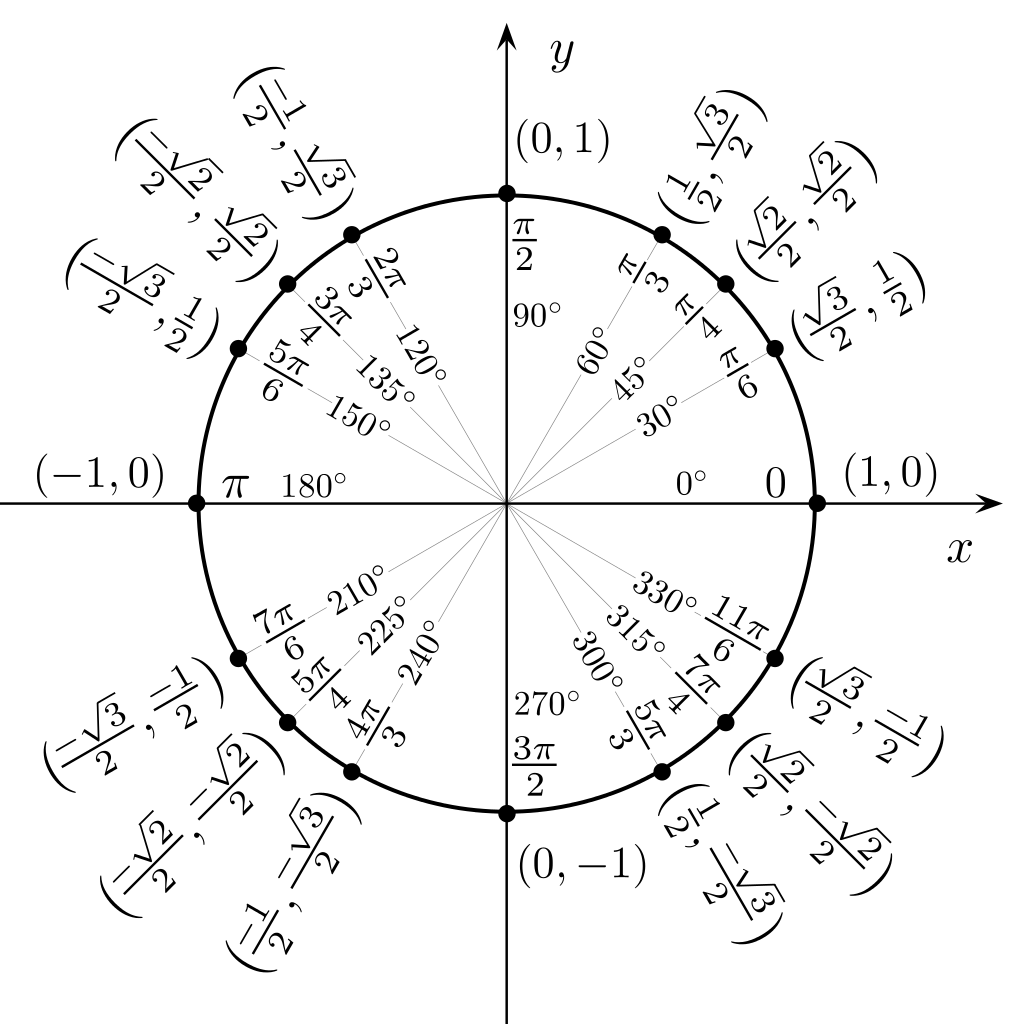
\includegraphics[width=0.3\textwidth]{Unit_circle_angles}
	
	\section{Indefinite Integrals}
	Taken from the ELEC 211 formula sheet\\
	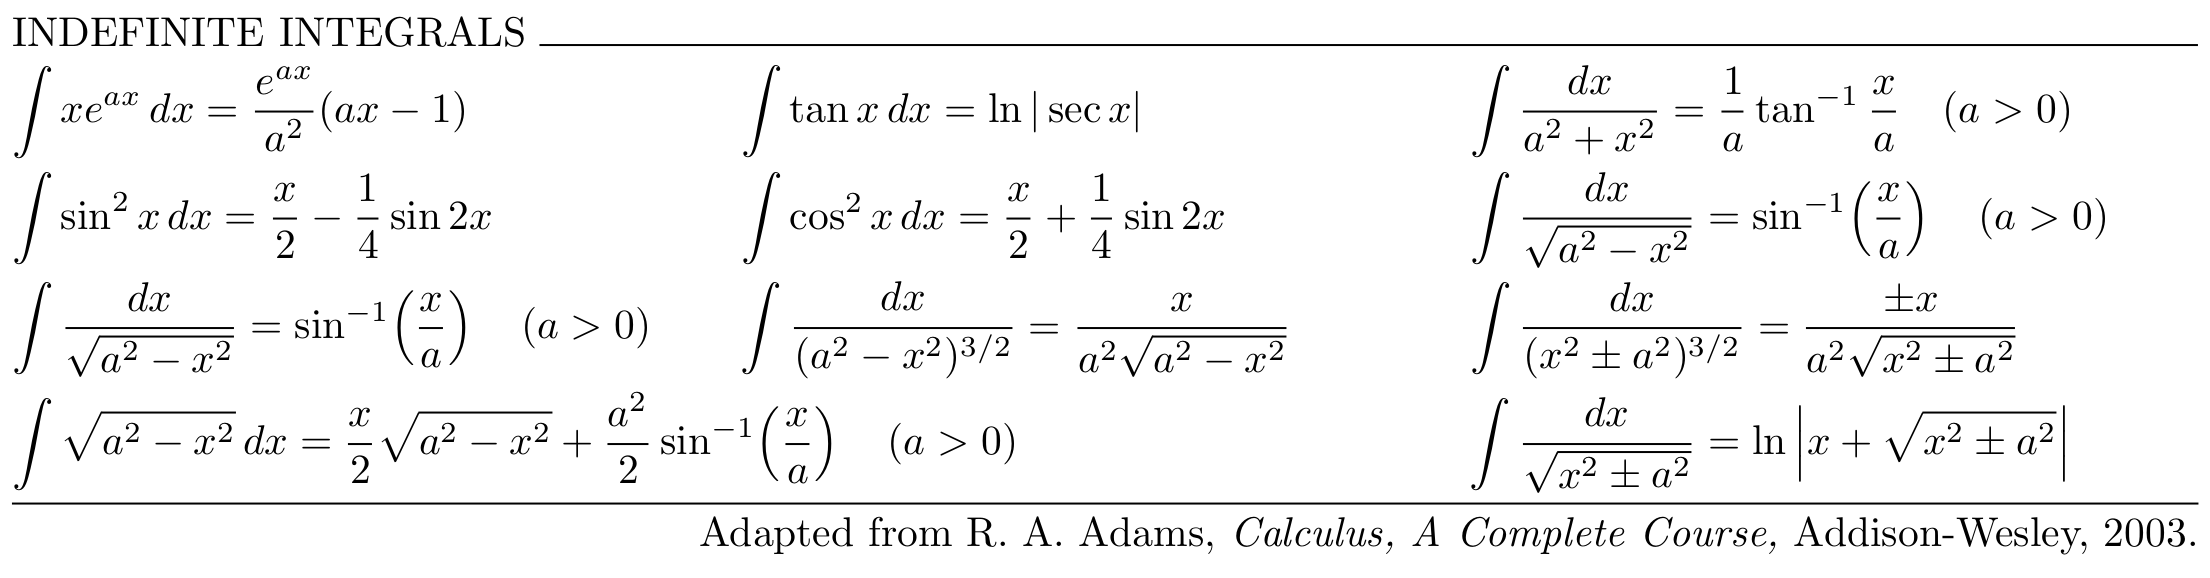
\includegraphics[width=0.6\textwidth]{indef-integrals}
	
	
\end{multicols*}

\newpage
\begin{multicols*}{2}
	\section{Fourier Transform Properties}
	\begin{tabularx}{0.5\textwidth}{|>{\raggedright\arraybackslash}X|>{\raggedright\arraybackslash}X|>{\raggedright\arraybackslash}X|}
		\hline
		& \textbf{Time} & \textbf{Frequency}\\
		\hline
		Linearity & $\alpha x(t) +\beta y(t)$ & $\alpha X(\omega) + \beta Y(\omega)$\\
		\hline
		Time scaling & $x(\alpha t), \alpha \neq 0$ & $\frac{1}{|\alpha |}X(\frac{\omega}{\alpha})$\\
		\hline
		Reflection & $x(-t)$ & $X(-\omega)$\\
		\hline
		Parseval's Energy Relation & $E_x = \int_{-\inf}^{\inf} |x(t)|^2 dt$ & $E_x = \frac{1}{2\pi}\int_{-\inf}^{\inf} |X(\omega)|^2 d\omega$\\
		\hline
		Duality & $X(t)$ & $2\pi x(-\omega)$\\
		\hline
		Time differentiation & $\frac{d^nx(t)}{dt^2}, n\ge 1$, integer & $(j\omega)^nX(\omega)$\\
		\hline
		Frequency differentiation & $-jtx(t)$ & $\frac{dX(\omega)}{d\omega}$\\
		\hline
		Integration & $\int_{-\inf}^{t}x(t')dt'$ & $\frac{X(\omega)}{j\omega}+\pi X(0)\delta (\omega)$\\
		\hline
		Time shifting & $x(t-\alpha)$ & $e^{-j\alpha \omega}X(\omega)$\\
		\hline
		Frequency shifting & $e^{j\omega_0 t}x(t)$ & $X(\omega - \omega_0)$\\
		\hline
		Modulation & $x(t)cos(\omega _c t)$ & $0.5|X(\omega - \omega _c) + X(\omega + \omega _c)|$\\
		\hline
		Periodic signals & $x(t) = \sum X_k e^{jk\omega_0 t}$ & $X(\omega) = \sum 2\pi X_k \delta (\omega - k\omega_0)$\\
		\hline
		Symmetry & $x(t)$ real & $|X(\omega)| = |X(-\omega)|$\\
		& & $\angle X(\omega)= -\angle X(-\omega)$\\
		\hline
		Windowing & $x(t)y(t)$ & $\frac{1}{2\pi}[X*Y](\omega)$\\
		\hline
		Cosine transform & $x(t)$ even & $X(\omega) = \int_{-\inf}^{\inf} x(t)cos(\omega t)dt$\\
		\hline
		Sine transform & $x(t)$ odd & $X(\omega) = -j\int_{-\inf}^{\inf} x(t)sin(\omega t)dt$\\
		\hline
	\end{tabularx}
\end{multicols*}

\end{document}
